\documentclass{beamer}
\usetheme{Singapore}
\usecolortheme{crane}
\usepackage{iwona}
\usepackage{tikz}
\usepackage{minted}

\beamertemplatenavigationsymbolsempty


\title{Refining a Plot With Matplotlib}
\author{Geraint Palmer}
\date{PyCon Namibia, 2016 \newline \href{http://na.pycon.org}{\tiny{http://na.pycon.org}}}

\begin{document}
\frame{\titlepage}

\begin{frame}
\frametitle{Anscombe's Quartet}
\begin{figure}
	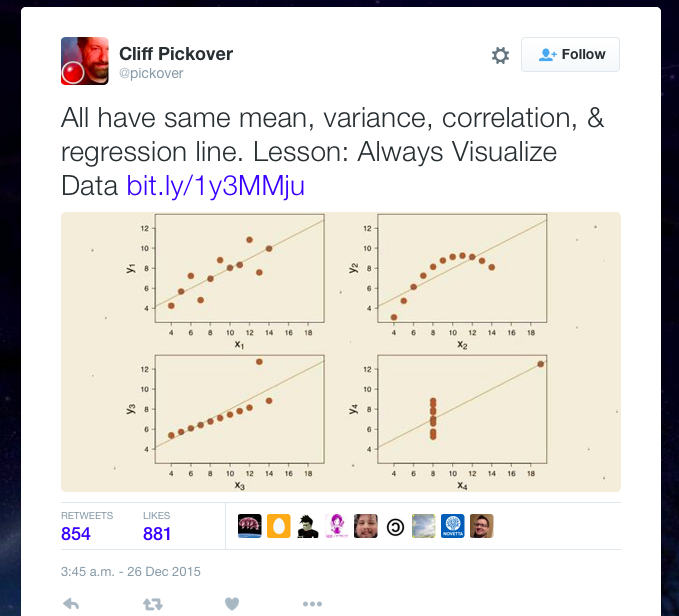
\includegraphics[width=0.65\textwidth]{anscombetweet}
\end{figure}
\end{frame}

\begin{frame}[fragile]
\begin{minted}{python}
import matplotlib.pyplot as plt
import seaborn as sns
sns.set(style="white")

fig, ax = plt.subplots()
plt.histogram(my_data)
plt.savefig('my_plot_name.png')
plt.show()
\end{minted}
\end{frame}

\begin{frame}
\frametitle{Histogram}
\begin{figure}
	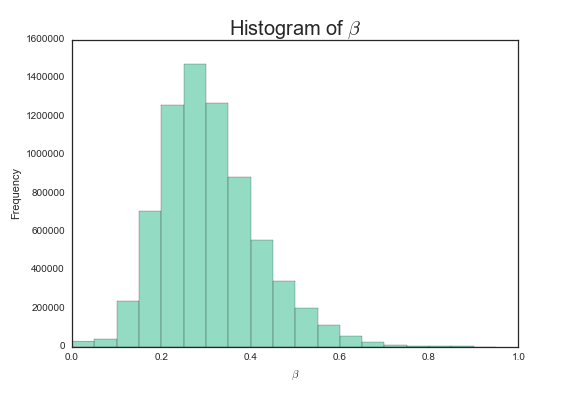
\includegraphics[width=\textwidth]{hist}
\end{figure}
\end{frame}

\begin{frame}
\frametitle{Overlayed Histogram}
\begin{figure}
	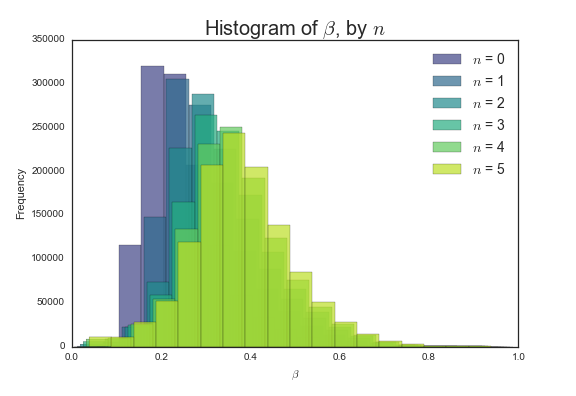
\includegraphics[width=\textwidth]{hist_overlay}
\end{figure}
\end{frame}

\begin{frame}
\frametitle{Stacked Histogram}
\begin{figure}
	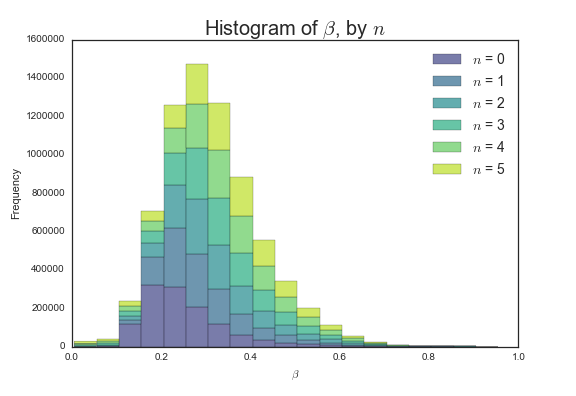
\includegraphics[width=\textwidth]{stacked_hist}
\end{figure}
\end{frame}

\begin{frame}[fragile]
\small{
\begin{minted}{python}
from scipy.stats import gaussian_kdesns.set(style="white")

densities = [gaussian_kde(row) for row in ratios_inverse_ns]
xs = [i/400.0 for i in range(400)]
ds = []
for dnsty in densities:
    dnsty.covariance_factor = lambda : 0.25
    dnsty._compute_covariance()
    ds.append(dnsty(xs))
\end{minted}
}
\end{frame}

\begin{frame}
\frametitle{Estimated PDF}
\begin{figure}
	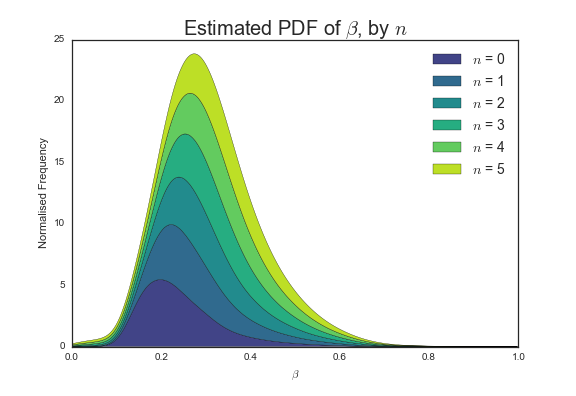
\includegraphics[width=\textwidth]{gaussian_1}
\end{figure}
\end{frame}

\begin{frame}
\frametitle{Estimated PDF}
\begin{figure}
	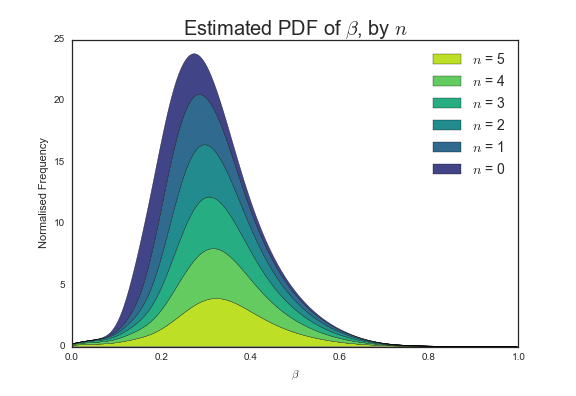
\includegraphics[width=\textwidth]{gaussian_2}
\end{figure}
\end{frame}

\begin{frame}
\frametitle{Line Plot}
\begin{figure}
	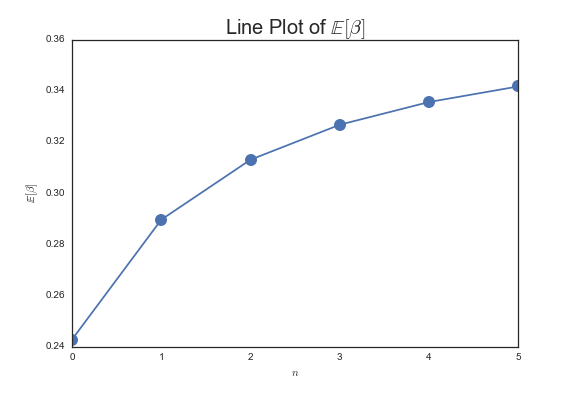
\includegraphics[width=\textwidth]{lineplotmeans}
\end{figure}
\end{frame}

\begin{frame}
\frametitle{2D Histogram}
\begin{figure}
	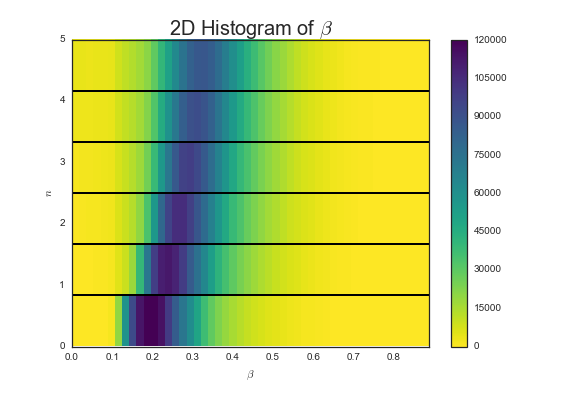
\includegraphics[width=\textwidth]{2dhist}
\end{figure}
\end{frame}

\begin{frame}
\frametitle{Violinplots \& Boxplots}
\begin{figure}
	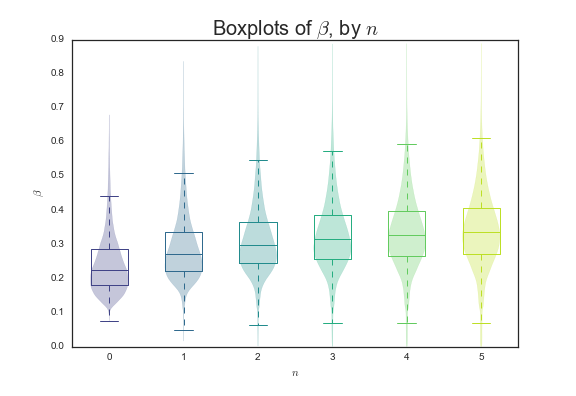
\includegraphics[width=\textwidth]{violins}
\end{figure}
\end{frame}

\end{document}